\chapter{DESENVOLVIMENTO}

Para \citeonline[p. 22]{minayo1994pesquisa}, “o conjunto de dados quantitativos e qualitativos não se opõem, ao contrário, se complementam.”Fica claro, então, que o objeto das Ciências Sociais é essencialmente qualitativo: a realidade social que “é o próprio dinamismo da vida individual e coletiva com toda a riqueza de significados dela transbordante.” \cite{minayo1994pesquisa}


\subsection{Tabela}

Tabelas podem ser criadas e inseridas facilmente com Latex. Elas podem ser personalidas. Colunas e linhas podem ser acrescentadas posteriormente. o Ajuste e flutuação pode ser indicado, entretant o Latex sempre procura a posição mais adequada.

\begin{table}[htb]
    \centering
    \caption{Pessoas residentes em domicílios particulares, por sexo e situação do domicílio – Brasil – 1980}
    \begin{tabular}{c c c c}
    \hline
        Situação do domicílio   & Total  &  Mulheres   &  Homens   \\
    \hline
        Total                   & 117.960.301 &  59.595.332 &  58.364.969 \\
        Urbana                  & 79.972.931  &  41.115.439 &  38.857.492 \\  
        Rural                   & 38.857.492  &  38.857.492 &  19.507.477 \\
    \hline
    \end{tabular}
    \fonte{Fundação Instituto Brasileiro de Geografia e Estatística - IBGE}
\end{table}


\subsection{Imagens}

A mesma flexibilidade aplicada para tabelas e gráficos pode ser empregada para introdução de imagens e figuras no texto. As boas práticas de uso do Latex indicam o uso de uma pasta determinada para guardar suas imagens e figuras.

\begin{fotografia}[htb]
 \IBGEtab{ %Comando nativo do pacote para geração dos labels das imagens e figuras
	\caption{Prática de Yoga na UNESC}
	\label{fot:grafico3}
 } {
  	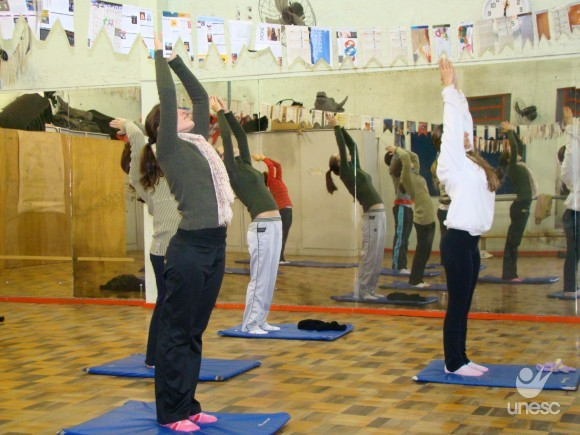
\includegraphics[scale=0.5]{figuras/yoga.png}
 } {
 	\fonte{Carrer (2004)}
 }
\end{fotografia}


